\subsection{Particle System} % (fold)
\label{sub:Particle System}
\subsubsection{研究背景}

一般2D 遊戲是利用 sprite 將一些靜態元素表現在螢幕上,若要做出角色移動這類的動畫效果,就會將很多 Sprite 組成 Sprite Sheet,接著去變換角色的 Sprite就能達到效果,像是這樣:

\begin{figure}[h]
    \begin{center}
    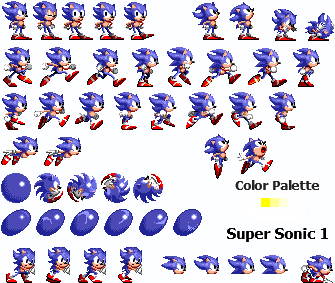
\includegraphics[width=0.5\textwidth]{./resources/particleSystem/example.png}
    \end{center}
\caption{Sprite Sheet示意圖}
\label{fig:particle_1}
\end{figure}

若需要一些特效,火焰、煙霧、煙火…等等,每個 Sprite 都需要請人畫,當東西複雜起來時這不會是個很好的方法。
因此我們需要一個能夠讓我們模擬各種不同效果的系統,而且只需要調參數就能讓我們快速的模擬各種不同的效果。

\subsubsection{實作}
這裡實作都以虛擬碼呈現

\subsubsection{Particle}

Particle 是粒子效果的基本單位,我們必須調整每個 particle 的位置、顏色、大小等等屬性以達到我們所要的效果

\begin{lstlisting}
struct Particle
{
    glm::vec2 pos;
    glm::vec2 startVel,endVel;
    glm::vec2 currentVel;
    float currentSize, startSize, endSize;
    float angle;
    float startRotSpeed;
    float currentRotSpeed;
    glm::vec4 startColor;
    glm::vec4 currentColor;
    glm::vec4 endColor;
    float t; // Timestep
    uint32_t startLife;
    uint32_t life;
};
\end{lstlisting}

\begin{itemize}
\item{pos}
    \SubItem{particle 目前的位置}
\item{startVel}
    \SubItem{particle 產生時的速度}
\item{currentVel}
    \SubItem{particle 目前的速度}
\item{endVel}
    \SubItem{particle 死亡時的速度}
\item{startSize}
    \SubItem{particle 產生時的大小}
\item{currentSize}
    \SubItem{particle 目前的大小}
\item{endSize}
    \SubItem{particle 死亡時的大小}
\item{angle}
    \SubItem{Particle Rotate的角度}
\item{startRotSpeed}
    \SubItem{Particle 起始旋轉速度}
\item{currentRotSpeed}
    \SubItem{Particle 目前旋轉速度}
\item{startColor}
    \SubItem{Particle 產生時的顏色}
\item{currentColor}
    \SubItem{Particle 目前的顏色}
\item{endColor}
    \SubItem{Particle 死亡的顏色}
\item{t}
    \SubItem{插值所用的 timestep}
\item{startLife}
    \SubItem{Particle 的生命週期}
\item{life}
    \SubItem{目前剩下的生命}
\end{itemize}

我們能夠設定每個 Particle 的初始、死亡的速度、大小、顏色等等,以達到Particle由快轉慢、由大轉小等效果、顏色由淺轉深等效果。

\subsubsection{Emitter}

Emitter 是定義 Particle 行為的地方,意思是說,如果我希望我的效果會讓粒子從紫色變黃色,我就要告訴 Emitter 我希望我的起始顏色是紫色,結束顏色是黃色。
接著當遊戲循環開始時,Emitter就會根據數據,將他給予到每個 Particle,讓他們模擬。

有了Emitter,當我們需要產生不同的效果,只需產生多個Emitter,給予不同的參數,就能有多個效果。Emitter擁有許多與Particle類似的數據。

\begin{lstlisting}
struct ParticleComponent
{
    glm::vec2 angleRange = {0.f, 360.f};
    float startSpeed = 0.f;
    float endSpeed = 0.f;
    float startSize = 0.f;
    float endSize = 0.f;
    float rotateSpeed = 0.f;
    int emissionRate = 0;
    uint32_t emitNumber = 0;
    uint32_t emitVariance = 0;
    uint32_t maxParticleLife = 0;
    uint32_t maxParticlesPerFrame = 0;
    int poolSize;
    bool active = false;
    float life = -1;
    float sleepTime;
    Timer lifeTimer;
    Timer sleepTimer;
    glm::vec4 startColor = {0, 0, 0, 0};
    glm::vec4 endColor = {0, 0, 0, 0};
    glm::vec2 rotSpeedRand = {0.f, 0.f};
    glm::vec2 startSpeedRand = { 0.f, 0.f};
    glm::vec2 endSpeedRand = {0.f, 0.f};
    glm::vec2 emitVarianceRand = {0.f, 0.f};
    glm::vec2 startSizeRand = {0.f, 0.f};
    glm::vec2 endSizeRand = {0.f, 0.f};
    glm::vec2 lifeRand = {0.f, 0.f};
    float disX = 0.f;
    float disY = 0.f;
    int lastUnusedParticle = 0;
    std::shared_ptr<Texture2D> texture;
    std::vector<Particle> particles;
};
\end{lstlisting}

\begin{itemize}
\item{angleRange}
    \SubItem{Particle 會在哪個角度反為裡排放}
\item{emissionRate}
    \SubItem{每個frame產生Particle的數量,由emitNumber跟emitVariance算出}
\item{emitNumber}
    \SubItem{每個frame保底產生Particle的數量}
\item{emitVariance}
    \SubItem{讓每個frame產生的數量不固定。此數會乘上一個介於(0, 1)範圍的值再加上 emitNumber來讓每個 frame 產生的數量不固定。}
\item{maxParticleLife}
    \SubItem{particle 的生命週期}
\item{maxParticlesPerFrame}
    \SubItem{用來計算 pool size}
\item{poolSize}
    \SubItem{particle pool 的大小}
\item{active}
    \SubItem{這個 Emitter 是否活著}
\item{life}
    \SubItem{Emitter 的生命週期。-1代表永久活著}
\item{sleepTime}
    \SubItem{每 sleepTime 產生一次 Particle}
\item{XXXRand}
    \SubItem{代表 XX 的random範圍,讓Particle看起來不會那麼整齊}
\item{disX/Y}
    \SubItem{disX, disY 用來決定paritcle產生的位置範圍}
\item{vector<Particle>}
    \SubItem{particle pool,這個 Emitter 所模擬的 particle}
\end{itemize}

\subsubsection{EmitData}
我們會將所有的數據放在外部,這樣更改數據之後並不需要重新編譯,也能重新選取檔案來快速切換效果。
\begin{lstlisting}
{
    "value0": {
        "angleRange": {
            "x": 250.0,
            "y": 280.0
        },
        "startSpeed": 200.0,
        "endSpeed": 200.0,
        "startSize": 0.0,
        "endSize": 80.0,
        "rotateSpeed": 0.0,
        "emitNumber": 3,
        ...
    }
}
\end{lstlisting}

\subsubsection{Particle System}

Particle System會模擬Particle的物理,以及幫助繪製粒子。
\begin{lstlisting}
class ParticleSystem
{
public:
    void update(Time dt, Emitter& emitter);
    void render(Emitter& emitter);
    void init(EmitData& data, Emitter& emitter);
}
\end{lstlisting}

選取想要的效果檔案後,能夠將讀取的資料傳給Particle System,並將資料輸入給Emitter

\begin{lstlisting}
void ParticleSystem::initEmitter(EmitData& data, Emitter& emitter) {
    emitter.angleRange = data.angleRange;
    emitter.startSpeed = data.startSpeed;
    emitter.endSpeed = data.endSpeed;
    emitter.startSize = data.startSize;
    emitter.endSize = data.endSize;
    emitter.rotateSpeed = data.rotateSpeed;
    /* ... */
}
\end{lstlisting}

Emitter 擁有資料之後,Particle System就能夠開始模擬例子效果了。

\begin{lstlisting}
void ParticleSystem::update(Time dt, Emitter& emitter) {
    if (emitter.active) {
        emitter.emissionRate = (int)(emitter.emitNumber + 
                emitter.emitVariance * randFloat(emitter.emitVarianceRand.x, emitter.emitVarianceRand.y));
        for(int i = 0 ; i < emitter.emissionRate ; i++) {
            int unusedParticle = firstUnusedParticle(emitter.lastUnusedParticle, emitter.particlePool);
            respawnParticle(emitter.particlePool, unusedParticle);
        }
    }
}
\end{lstlisting}

更新的時候,首先確認此 Emitter 是否存活(emitter.active)如果存活,計算出這一個 frame 要產生多少個 particle(emitter.emissionRate),然後激活emissionRate數量的粒子。

激活粒子方法呢,會在我們的 Particle pool 中,找到未被使用的粒子並將它激活。

\begin{lstlisting}
uint32_t ParticleSystem::firstUnusedParticle(uint32_t &lastUnusedParticle, vector<Particle>& particlePool) {
    for(int i = lastUnusedParticle ; i < particlePool.size() ; i++) {
        if(particlePool[i].life <= 0) {
            lastUnusedParticle = i;
            return i;
        }
    }

    for(int i = 0 ; i < lastUnusedParticle ; i++) {
        if(particlePool[i].life <= 0) {
            lastUnusedParticle = i;
            return i;
        }
    }
    lastUnusedParticle = 0;
    return lastUnusedParticle;
}
\end{lstlisting}

激活就是將Emitter的數據給予每個Partcle
當每個Particle都擁有了數據以及生命之後,就能來更新他的數據了。

\begin{lstlisting}
/* .... */

for(int i = 0 ; i < emitter.poolSize ; i++) {
    auto &particle = emitter.particles[i];
    if(particle.life > 0.f) {
        particle.currentSize = interpolateBetweenRange(particle.startSize, particle.t, particle.endSize);
        particle.currentVel.x = interpolateBetweenRange(particle.startVel.x, particle.t, particle.endVel.x);
        particle.currentVel.y = interpolateBetweenRange(particle.startVel.y, particle.t, particle.endVel.y);
        particle.currentColor = RGBAinterpolation(particle.startColor, particle.t, particle.endColor);

        particle.pos.x += particle.currentVel.x * dt;
        particle.pos.y += particle.currentVel.y * dt;
        particle.life--;

        particle.t += (1.0f/(float)particle.startLife);
        if(particle.t >= 1.f)
            particle.t = 0.f;

        particle.currentRotSpeed += particle.startRotSpeed;
        particle.angle += dt * particle.currentRotSpeed;
        particle.angle = fmod(particle.angle, 360.f);
    }
}
\end{lstlisting}

如果那顆粒子是活的,我們就更新它。 利用插值法更新速度、大小以及顏色。
然後根據速度以及這一個 frame 經過的時間更新 Particle 的位置

\subsubsection{Vortex}

Vortex,渦流,類似一種像漩渦般不斷旋轉的空氣,而我們的Particle會被這個旋轉的空氣影響,進而影響行走的路徑。可以想像有個隱形的颱風在螢幕上,而每個直走的Particle會因為經過颱風而往右邊或左邊走。

Particle 會受 Vortex 的位置(pos)、旋轉速度(speed)以及大小(size)影響。

\begin{lstlisting}
struct Vortex {
    glm::vec2 pos = {0.f, 0.f};
    float speed = 0.f;
    float size = 0.f;
}
\end{lstlisting}

擁有這些數據後,我們更改 Particle System 裡 Particle 的更新方法。

\begin{lstlisting}
float dx = particle.pos.x - vortex.pos.x;
float dy = particle.pos.y - vortex.pos.y;
float vx = -dy * vortex.turbulence.x;
float vy = dx * vortex.turbulence.y;
factor_ = 1.0f/ (1.0f + (dx*dx + dy*dy)/vortex.currentSize*0.1);

particle.pos.x += (vx - particle.currentVel.x) * factor_ + particle.currentVel.x * dt;
particle.pos.y += (vy - particle.currentVel.y) * factor_ + particle.currentVel.y * dt;
\end{lstlisting}

這種 Vortex 是固定不動的,如果希望 Vortex 也會跟著移動的話,只需要將 Vortex 當作另一種 Particle 一起排放。

動態的 Vortex 影響 Particle 的方法:

\begin{lstlisting}
factor_ = 1.0f / (1.0f + (dx*dx + dy*dy) / (vortex.currentSize * 0.1));
float lifeFactor = vortex.life / emitter.vortexMaxParticleLife;
factor_ *= (1-lifeFactor) * lifeFactor * 4;
\end{lstlisting}

Vortex 隨著時間移動,也會隨著時間消失,而在 Vortex 快死亡時對 Partcle 的影響逐漸減少。


\begin{figure}[h]
    \begin{subfigure}[b]{0.5\linewidth}
        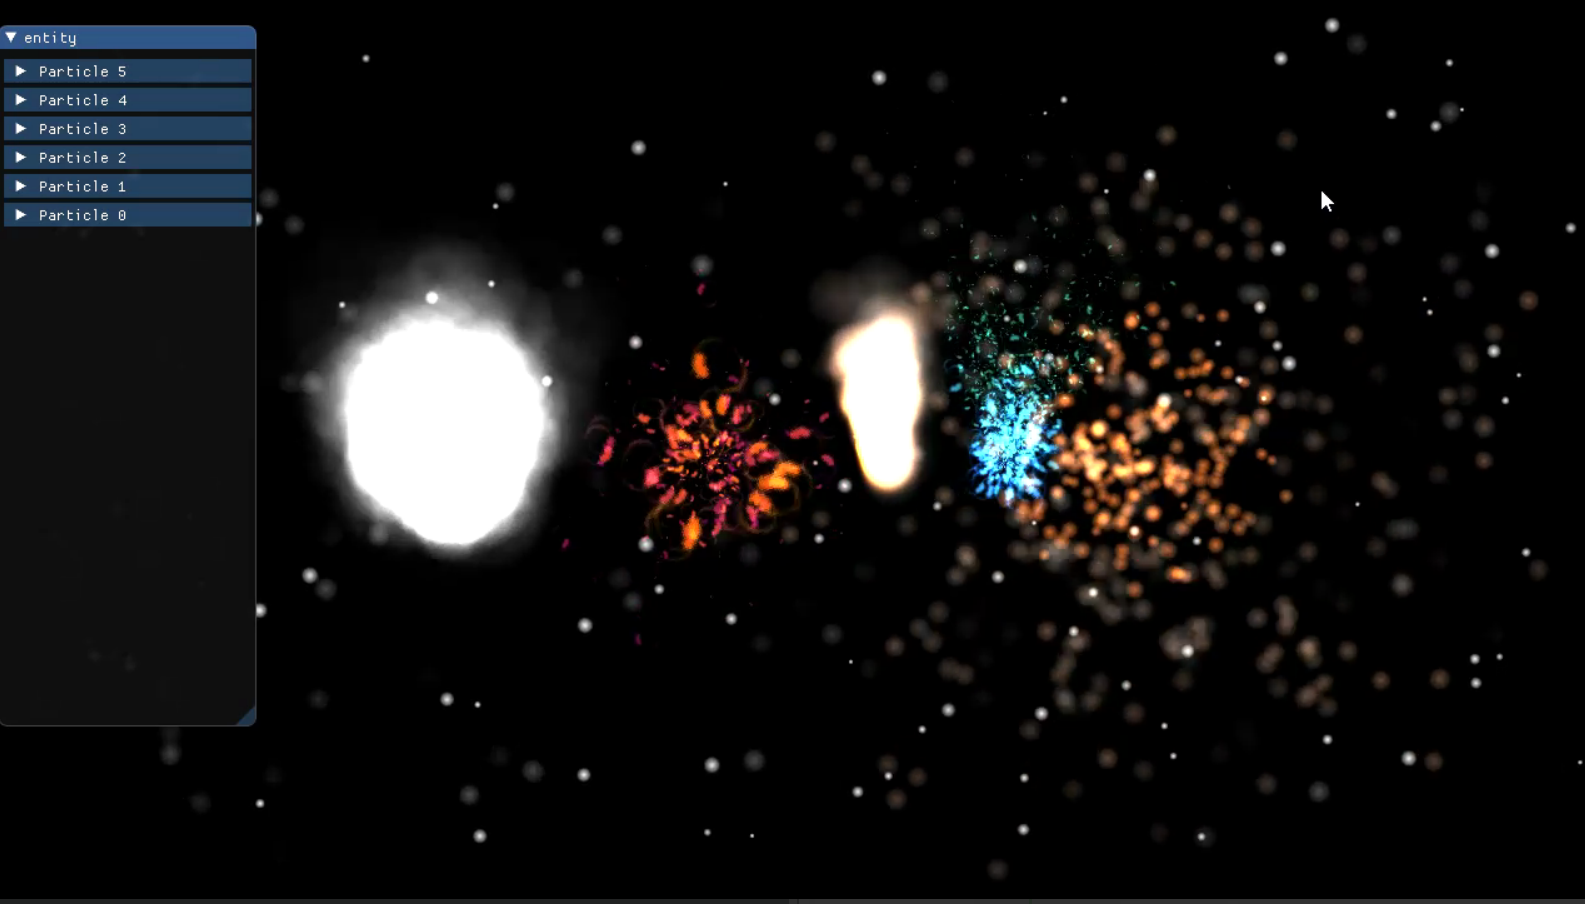
\includegraphics[width=\linewidth]{./resources/particleSystem/particle.png}
        \caption{Particle}
    \end{subfigure}
    \begin{subfigure}[b]{0.5\linewidth}
        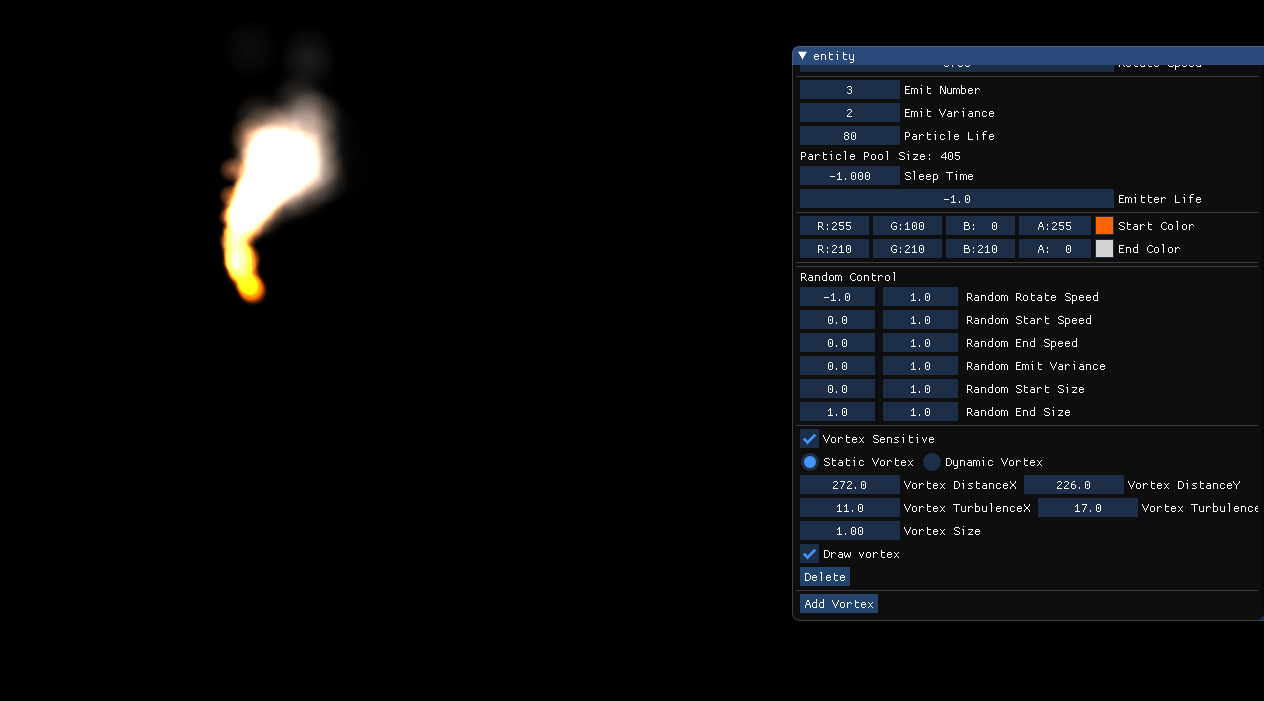
\includegraphics[width=\linewidth]{./resources/particleSystem/vortex.png}
        \caption{Vortex}
    \end{subfigure}
\caption{Particle System 模擬}
\label{fig:simulate}
\end{figure}

% \subsubsection{結論}

% 目前這個Particle System能夠做出像是煙霧、煙火、火焰、雪等效果,各種其他特效也能透過條參數來獲得效果,且還能控制排放的間隔,每多少秒才排放一次。
% 未來希望能夠新增更多的 particle 排放的曲線,不只能夠調整參數,能夠有個函數圖形讓使用者們直接選取中意的曲線,來模擬particle的路徑。

\newpage
